\pattern{Client Server}
\begin{summary}
    The client-server architecture is a pure network architecture in which each
    computer or process on the network is either a client or a server. There
    are 3 major components. First we have the servers which are powerful
    computers or processes dedicated to managing disk drives (file servers),
    printers (print servers), or network traffic (network servers). Second,
    clients are workstations on which users can run applications. Finally we
    have resources which are files, devices, and even processing power. The
    components are connected via connectors which are essentially network layer
    protocols such as TCP/IP.
\end{summary}

\comparison{\begin{itemize}

        \item The architecture style allows the system to distribute workload
            amongst multiple machines or processes. It is very flexible as to
            allow the architect to decide how to divide tasks amongst the
            clients and servers. This helps promote the separation of concerns.
            The architecture style is most beneficial when increasing the
            modularity of the components and decreasing coupling. This can be
            done through encapsulation of information with a well-defined
            standardized interface. The system will also allow centralized
            control and redesign since all machines and processes should be
            running software defined by the system architect.

\end{itemize}
}{\begin{itemize}
        \item Due to its centralized design, need load-balancer and failover
            systems in order to scale properly. There is a possibility for
            congestion of traffic, which motivates the need for the
            load-balancers. A client-server network is also costly to set up,
            often requiring you to purchase licenses like a copy of Windows NT,
            which is a family of operating systems for servers, and also client
            licenses. The hardware required for servers is also needed to be
            more powerful than a standard workstation, and additionally require
            employees to manage them. This means paying more for equipment and
            networking professionals, who don’t come cheap, to even run the
            server.

        \item The client-server system is especially vulnerable to failures as
            there is always going to be a limited number of servers relative to
            clients. If a critical number of them go down, no users will be
            able to use the system until the servers are fixed or replaced.
            This makes them vulnerable to denial of service attack, distributed
            denial of service attack where the perpetrator seeks to make a
            machine or network resource unavailable to its intended users by
            temporarily or indefinitely disrupting services of a host connected
            to the Internet. Denial of service is typically accomplished by
            flooding the targeted machine or resource with superfluous requests
            in an attempt to overload systems
\end{itemize}}

\begin{nfps}
\item[Dependability] The architecture supports availability as servers are easy
    to keep running and typically do not have to shutdown or restart for many
    days. It also supports dependability as control and distribution of
    resources and data are controlled by a dedicated server. 
\item[Heterogeneity] clients and servers often function as disparate parts. 
\item[Scalability] the centralized servers can be updated with minimal impact
    to the client.

\item[Negative Efficiency] since the server handles all the stress and demand
    of the system. When there is an unanticipated amount of stress and the
    server becomes congested, performance can slow down drastically or even
    fail to perform which affects all users. 
\item[Negative Transparency?] It also inhibits transparency because
    communication is restricted to requests and clients are unable to see fetch
    processes running on the server.
\end{nfps}

\subsubsection{Implementation and Example}

As seen from the diagrams, the flow of the data is unidirectional and forms a
cycle. It is usually initiated by the client requesting some kind of data and
the server processing the request and sending some kind of data back to the
client. A typical topological data flow goes as follows:
\begin{enumerate}[noitemsep]
    \item Client request data from server
    \item Load balancer routes the request to the appropriate server
    \item Server process the request client
    \item Server queries appropriate database for some data
    \item Database return the queried data back the server
    \item The server processes the data and send the data back to the client
    \item (This process repeats)
\end{enumerate}

All technology companies today use this architecture, Uber, Facebook, Airbnb,
etc.
\begin{center}
    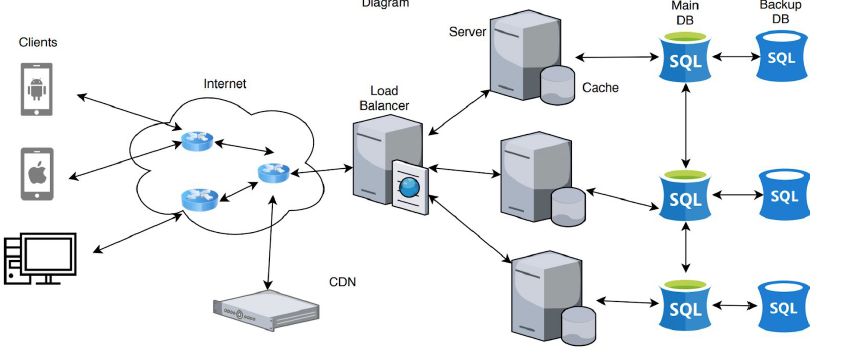
\includegraphics[width=0.4\textwidth]{./client-server}
\end{center}
